\documentclass[11pt,a4paper,twocolumn]{article}

% === Core Packages ===
\usepackage[margin=2cm]{geometry}
\usepackage[utf8]{inputenc}
\usepackage[T1]{fontenc}
\usepackage{times}
\usepackage{amsmath,amssymb}
\usepackage{graphicx}
\usepackage{booktabs}
\usepackage{float}
\usepackage{enumitem}
\usepackage{tikz}
\usepackage{pgfplots}
\pgfplotsset{compat=1.18}
\usetikzlibrary{arrows.meta,shapes.geometric,positioning,calc,decorations.markings,fit,backgrounds}

% === Citation (IEEE style) ===
\usepackage[numbers,sort&compress]{natbib}
\bibliographystyle{IEEEtranN}

% === Hyperref ===
\usepackage[hidelinks]{hyperref}
\usepackage{xurl}

% === Settings ===
\setlength{\parindent}{1em}
\setlength{\parskip}{0.3em}

% === PDF metadata ===
\hypersetup{
  pdftitle={Rede de Reputação Descentralizada: Um Modelo para a Organização Natural da Sociedade},
  pdfauthor={Pavel Kudrna},
  pdfsubject={Personix — a decentralized reputation network},
  pdfkeywords={Personix, decentralized reputation, reputation social network,
    decentralized identifiers, DID, meritocracy, censorship resistance},
}

% === Title ===
\title{\textbf{Rede de Reputação Descentralizada:\\Um Modelo para a Organização Natural da Sociedade}}
\author{Pavel Kudrna\\Personix Project --- \url{https://personix.org}\\Prague, Czechia\\Rascunho v1 --- Março de 2026}
\date{}

\begin{document}
\maketitle

% ============================================================
% ABSTRACT
% ============================================================
\begin{abstract}
O sentido de justiça---a convicção de que os agravos são reparados e o mérito é recompensado---é a mais forte força de coesão da sociedade. Quando as instituições centralizadas de governação não conseguem proporcionar este sentido, porque o custo de fazer valer um direito excede o próprio valor desse direito, a coesão social erode-se. As estruturas institucionais actuais falham na resolução de uma classe significativa de litígios sistematicamente da mesma forma que o planeamento central falha na afectação de recursos: através da assimetria de informação, da ausência de mecanismos de retroacção e da desconexão entre os decisores e as consequências das suas decisões. Este artigo apresenta uma Rede Social de Reputação (RSN): uma camada de comunicação descentralizada, incorruptível e resistente à censura, construída sobre Identificadores Descentralizados (DIDs), que permite a participantes pseudónimos publicar, verificar e consumir informação de reputação sobre comportamento no mundo real. O mecanismo central assenta em três princípios de conceção: (1)~uma estrutura de custos assimétrica em que ler dados de reputação é barato mas escrever exige um esforço verificável; (2)~um protocolo não determinístico de seleção de verificadores baseado em hashing consistente, que fixa o preço de alegações radicais através de custos de iteração crescentes; e (3)~um modelo de autoridade de reputação orientado pelo mercado, em que verificadores privados apostam a reputação acumulada na exatidão das alegações que endossam. A arquitetura resultante produz uma meritocracia emergente sem coordenação central e possibilita um caminho de migração gradual e reversível a partir dos sistemas actualmente administrados pelo Estado.
\end{abstract}

% ============================================================
% 1. INTRODUCTION
% ============================================================
\section{Introdução}

\subsection{O Problema da Confiança Centralizada}

A governação moderna assenta num pressuposto fundamental: o de que as instituições centralizadas conseguem mediar a confiança entre desconhecidos em larga escala. Os tribunais julgam litígios. Os registos certificam a propriedade. Os organismos reguladores fazem cumprir normas. Estas instituições foram concebidas numa era em que a informação era escassa, a comunicação era lenta e a delegação de autoridade num corpo central era o único mecanismo de coordenação viável. A governação centralizada, contudo, falha pelas mesmas razões estruturais que o planeamento central: assimetria de informação, ausência de mecanismos de retroacção e desconexão entre os decisores e as consequências das suas decisões.

O pressuposto falha, por exemplo, quando o custo da mediação institucional excede o valor do litígio. Considere-se um inquilino que descobre que o apartamento arrendado carece de um certificado de segurança elétrica legalmente exigido---uma condição que representa perigo imediato para a vida. O direito legal do inquilino a rescindir o contrato é inequívoco. Contudo, o custo de fazer valer esse direito através do sistema judicial excede o valor monetário da caução e dos danos devidos, mesmo incluindo a eventual compensação legal~\cite{czcourtfees}. A resposta racional é absorver a perda e sair.

Este não é um caso patológico e excecional. É a experiência habitual para uma classe significativa de litígios em que o dano é real mas os valores monetários em jogo ficam abaixo do limiar a partir do qual a execução institucional se torna economicamente racional. O resultado é um sistema que favorece estruturalmente os maus atores: quem prejudica os outros em montantes abaixo deste limiar pode agir impunemente, porque o custo de procurar justiça recai sobre a parte lesada.

O exemplo acima é retirado do enquadramento jurídico do autor---o sistema checo de direito civil. Noutras tradições jurídicas---direito comum baseado em precedente, direito consuetudinário, sistemas mistos---a justiça falha de formas diferentes e em graus diferentes, consoante as especificidades culturais e processuais da jurisdição. Os leitores reconhecerão provavelmente exemplos equivalentes no seu próprio contexto. O que é estruturalmente universal é o padrão: litígios cujo valor fica abaixo do limiar de execução economicamente racional terminam com a perda a ser absorvida pela parte lesada. A RSN não promete uma justiça perfeita---limita-se a reduzir a vantagem estrutural de que os maus atores gozam quando a execução institucional não é economicamente viável.

\subsection{Porque as Soluções Existentes Ficam Aquém}

\textbf{Os modelos de Identidade Descentralizada (DID)}~\cite{did2022} fornecem mecanismos criptográficos para a gestão autossoberana de identidade, mas centram-se sobretudo na verificação de identidade sem abordar a questão mais ampla da reputação comportamental.

\textbf{Os Soulbound Tokens (SBTs)}~\cite{weyl2022} captam a ideia de que a reputação é intransferível, mas dependem de infraestrutura blockchain com limitações de escalabilidade e não abordam os incentivos económicos que regem a entrada de informação. Conceitos relacionados, como os tokens de mérito (p.\,ex., Liberland), partilham uma filosofia semelhante mas permanecem vinculados a enquadramentos jurisdicionais específicos.

\textbf{As Organizações Autónomas Descentralizadas (DAOs)}~\cite{buterin2014} implementam governação através de contratos inteligentes, mas replicam dinâmicas plutocráticas em que a influência é proporcional ao capital. O voto quadrático~\cite{buterin2019} atenua parcialmente este problema mas limita a adoção prática. As DAOs enfrentam também o \emph{problema do oráculo} fundamental: os contratos inteligentes não conseguem verificar de forma fiável estados do mundo real sem uma fonte externa de confiança, e este problema não tem solução geral no âmbito da arquitetura blockchain.

Nenhum sistema existente combina descentralização, resistência à censura, pseudonímia, custo de entrada verificável e consenso emergente.

\subsection{Contribuições}

Este artigo apresenta as seguintes contribuições:
\begin{enumerate}[nosep]
\item A definição da \textbf{Rede Social de Reputação (RSN)}, um protocolo descentralizado que estende o modelo DID para suportar a troca bilateral de reputação.
\item Um \textbf{protocolo não determinístico de seleção de verificadores} baseado em hashing consistente~\cite{karger1997}.
\item O \textbf{Princípio do Radicalismo Dispendioso}, que fixa o preço das alegações consoante a sua distância ao consenso da rede através de três canais de custo cumulativos.
\item Um \textbf{modelo de Autoridade Reputável} com incentivos assimétricos, em que o endosso falso custa catastroficamente mais do que os emolumentos legítimos.
\item Um \textbf{caminho de migração gradual} através de uma infraestrutura fiscal paralela.
\end{enumerate}

% ============================================================
% 2. DESIGN PRINCIPLES
% ============================================================
\section{Princípios de Conceção}

A arquitetura da RSN é condicionada por cinco princípios de conceção inegociáveis.

\textbf{Continuidade e Evolução.} O sistema coexiste com as instituições existentes durante um período de transição de duração indefinida. A transição tem de ser reversível em todas as fases.

\textbf{Voluntariedade e Responsabilidade.} A participação é voluntária, mas a voluntariedade está associada à responsabilidade: um participante que assume o controlo de uma função institucional assume simultaneamente as obrigações que a acompanham.

\textbf{Diversidade e Neutralidade Cultural.} O consenso emerge das interações bilaterais, e não de regras predefinidas impostas pelos conceptores do sistema.

\textbf{Resiliência e Resistência à Censura.} O custo de censurar a rede tem de exceder o custo de a tolerar. Só um totalitarismo pleno---a um custo político e económico ruinoso---pode suprimir o sistema.

\textbf{Consenso e Execução.} O sistema incorpora as tendências humanas para a mesquinhez, o rancor e a satisfação retributiva como elementos estruturais. A má conduta não é proibida; tem um preço.

% ============================================================
% 3. SYSTEM OVERVIEW
% ============================================================
\section{Visão Geral do Sistema}

\subsection{Rede Social de Reputação}

A RSN é uma camada de comunicação descentralizada e ponto a ponto na qual os participantes trocam informação verificável sobre comportamento no mundo real. As suas propriedades definidoras são: infraestrutura descentralizada e incensurável; participação pseudónima através de DIDs; estrutura de custos assimétrica (ler é barato, escrever é dispendioso); verificabilidade criptográfica; e \textbf{suporte a normas}---formatos legíveis por máquina para a informação propagada através da rede, para os serviços oferecidos pelas autoridades (composição de alegações, endosso, serviço de testemunho) e para o formato de política, incluindo as regras de avaliação da reputação da contraparte e a estimativa do risco de discrepância de política (entre o comportamento declarado e o real).

\subsection{Componentes Arquiteturais}

A RSN é constituída por quatro componentes principais (Fig.~\ref{fig:architecture}):
\begin{enumerate}[nosep]
\item \textbf{Camada DID.} Identidades dos participantes com regras declaradas, metadados de reputação e encaminhamento na rede.
\item \textbf{Protocolo de Alegações.} Formato estruturado para publicar asserções sobre acontecimentos do mundo real.
\item \textbf{Rede de Verificação.} Protocolo descentralizado para atribuir verificadores mediante hashing consistente.
\item \textbf{Camada de Agregação de Reputação.} Serviços que produzem resumos de reputação legíveis por humanos.
\end{enumerate}

\begin{figure}[ht]
\centering
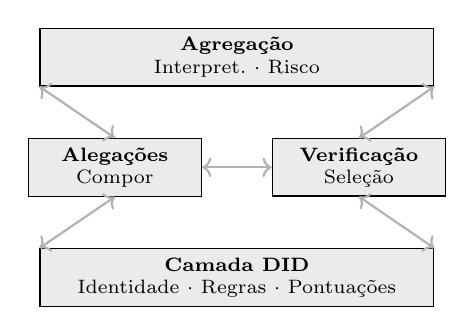
\begin{tikzpicture}[
    layer/.style={draw, minimum height=0.7cm, align=center, font=\scriptsize, fill=black!8},
    arr/.style={<->, thick, gray!60}
]
\node[layer, minimum width=5cm] (agg) at (0,2.8) {\textbf{Agregação}\\Interpret.\ $\cdot$ Risco};
\node[layer, minimum width=2.2cm] (claim) at (-1.55,1.4) {\textbf{Alegações}\\Compor};
\node[layer, minimum width=2.2cm] (verif) at (1.55,1.4) {\textbf{Verificação}\\Seleção};
\node[layer, minimum width=5cm] (did) at (0,0) {\textbf{Camada DID}\\Identidade $\cdot$ Regras $\cdot$ Pontuações};

\draw[arr] (agg.south west) -- (claim.north);
\draw[arr] (agg.south east) -- (verif.north);
\draw[arr] (claim.east) -- (verif.west);
\draw[arr] (claim.south) -- (did.north west);
\draw[arr] (verif.south) -- (did.north east);
\end{tikzpicture}
\caption{Arquitetura da RSN em quatro camadas.}
\label{fig:architecture}
\end{figure}

\subsection{Papéis dos Participantes}

Uma transação de verificação envolve até seis papéis DID distintos (Fig.~\ref{fig:roles}): \textbf{Emissor} ($DID_I$, cria e submete a alegação), \textbf{Sujeito} ($DID_S$, o DID a que a alegação diz respeito---pode coincidir com o Emissor), \textbf{Autoridade} ($DID_A$, endossa a alegação mediante emolumentos; pode também oferecer serviços de testemunho---\emph{opcional}), \textbf{Testemunha} ($DID_{W_{1..n}}$, monitor incógnito da honestidade do verificador através de códigos de desafio---\emph{opcional}), \textbf{Verificador} ($DID_V$, selecionado algoritmicamente para publicar a alegação) e a \textbf{RSN} (a rede onde as alegações verificadas são publicadas). Qualquer papel pode ser delegado noutro DID (Secção~7.4). Uma Autoridade combina frequentemente o endosso com serviços de testemunho, mas as duas funções são logicamente independentes.

\begin{figure}[ht]
\centering
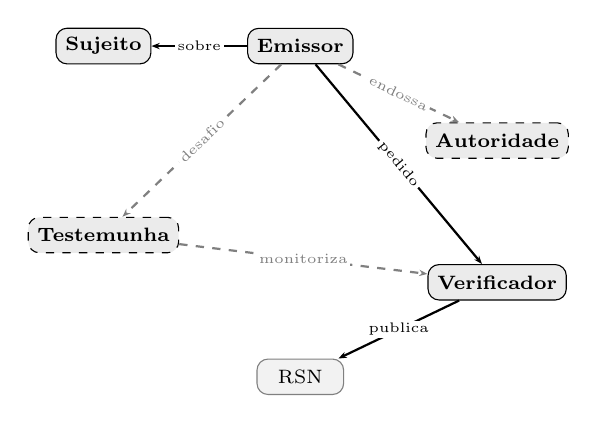
\begin{tikzpicture}[
    role/.style={draw, rounded corners, minimum width=1.1cm, minimum height=0.45cm, align=center, font=\scriptsize, fill=black!8},
    opt/.style={draw, rounded corners, minimum width=1.1cm, minimum height=0.45cm, align=center, font=\scriptsize, fill=black!8, dashed},
    arr/.style={-{Stealth[length=3pt]}, thick},
    oarr/.style={-{Stealth[length=3pt]}, thick, dashed, gray},
    lbl/.style={font=\tiny, fill=white, inner sep=1pt}
]
\node[role] (I) at (0,2.4) {\textbf{Emissor}};
\node[role] (S) at (-2.5,2.4) {\textbf{Sujeito}};
\node[opt] (A) at (2.5,1.2) {\textbf{Autoridade}};
\node[opt] (W) at (-2.5,0) {\textbf{Testemunha}};
\node[role] (V) at (2.5,-0.6) {\textbf{Verificador}};
\node[role, fill=black!5, draw=gray] (N) at (0,-1.8) {RSN};

\draw[arr] (I) -- node[lbl] {sobre} (S);
\draw[oarr] (I) -- node[lbl,sloped] {endossa} (A);
\draw[oarr] (I) -- node[lbl,sloped] {desafio} (W);
\draw[arr] (I) -- node[lbl,sloped] {pedido} (V);
\draw[oarr] (W) -- node[lbl] {monitoriza} (V);
\draw[arr] (V) -- node[lbl] {publica} (N);
\end{tikzpicture}
\caption{Papéis DID numa transação de verificação. Tracejado = opcional (Autoridade, Testemunha).}
\label{fig:roles}
\end{figure}

\subsection{Incorruptibilidade: Quatro Forças}

A incorruptibilidade da RSN não decorre de um único mecanismo, mas de quatro forças concorrentes. Nenhuma é suficiente por si só; só a sua combinação torna economicamente irracional qualquer tentativa de corrupção.

\textbf{Alvo imprevisível.} O verificador de cada alegação é selecionado de forma não determinística através de hashing consistente (Secção~5.3). Um atacante não pode escolher previamente um verificador específico para suborno, porque a identidade do verificador é função do conteúdo da alegação e das iterações anteriores, e não da escolha do emissor.

\textbf{Alavancagem reputacional---subida lenta, queda rápida.} A reputação só pode ser adquirida de forma incremental, através de um comportamento consistente e sustentado. Pode, contudo, ser perdida de forma catastrófica num único endosso fraudulento (Secção~6.2). Esta assimetria significa que anos de reputação acumulada podem ser destruídos por um único endosso desonesto; a estratégia ótima continua a ser rejeitar alegações suspeitas.

\textbf{Promessa pública.} Cada Titular de DID declara publicamente a sua política---um conjunto de regras legíveis por máquina que se compromete a cumprir. A divergência entre a declaração e o comportamento real é detetável e tem um preço, como uma infração reputacional mais grave do que a violação subjacente (Secção~7.3). A hipocrisia é, por isso, mais dispendiosa do que a desonestidade direta.

\textbf{Assimetria do custo de ataque em malha.} O custo de censurar ou desestabilizar a rede cresce de forma não linear com a dimensão e a densidade da rede, ao passo que o custo de a tolerar permanece constante. Para que a censura compensasse, um ator centralizado teria de a aplicar a toda a rede---exigindo medidas desproporcionadas face a qualquer benefício concebível (Secção~10).

% ============================================================
% 4. DECENTRALIZED IDENTITY MODEL
% ============================================================
\section{Modelo de Identidade Descentralizada}

\subsection{DID com Propriedades Especiais}

A RSN estende a especificação W3C DID Core~\cite{did2022} com: \textbf{Regras Declaradas} (compromissos comportamentais legíveis por máquina), \textbf{Metadados de Reputação} (pontuação comportamental agregada) e \textbf{Encaminhamento na Rede} (gateway onion mutável, separado da posição estável no anel).

\subsection{Ciclo de Vida da Alegação}

Uma Alegação percorre seis etapas (Fig.~\ref{fig:lifecycle}): composição, endosso opcional por uma autoridade, seleção do verificador via hashing consistente, decisão de verificação (aceitar ou rejeitar com iteração), publicação e atualização de reputação para todas as partes.

\begin{figure}[ht]
\centering
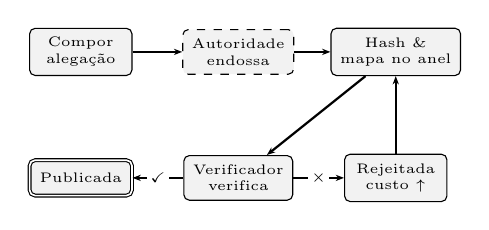
\begin{tikzpicture}[
    stp/.style={draw, rounded corners=2pt, minimum width=1.3cm, minimum height=0.45cm, align=center, font=\tiny, fill=black!5},
    arr/.style={-{Stealth[length=3pt]}, thick},
    lbl/.style={font=\tiny, fill=white, inner sep=1pt}
]
\node[stp] (comp) at (0,0) {Compor\\alegação};
\node[stp, dashed] (auth) at (2.0,0) {Autoridade\\endossa};
\node[stp] (hash) at (4.0,0) {Hash \&\\mapa no anel};
\node[stp] (ver) at (2.0,-1.6) {Verificador\\verifica};
\node[stp, double] (pub) at (0,-1.6) {Publicada};
\node[stp] (rej) at (4.0,-1.6) {Rejeitada\\custo $\uparrow$};

\draw[arr] (comp) -- (auth);
\draw[arr] (auth) -- (hash);
\draw[arr] (hash) -- (ver);
\draw[arr] (ver) -- node[lbl] {\checkmark} (pub);
\draw[arr] (ver) -- node[lbl] {$\times$} (rej);
\draw[arr] (rej) -- ++(0,0.8) -| (hash);
\end{tikzpicture}
\caption{Ciclo de vida da alegação com laço de iteração.}
\label{fig:lifecycle}
\end{figure}

\subsection{Relação com a W3C DID Core}

O modelo de identidade da RSN é um superconjunto próprio da especificação W3C DID Core~\cite{did2022}. Todos os DIDs da RSN são DIDs W3C válidos. As extensões específicas da RSN são codificadas como propriedades do documento DID definidas numa especificação de método DID dedicada, compatível com infraestruturas existentes como a ION~\cite{buchner2021} e a Ceramic~\cite{ceramic2023}.

% ============================================================
% 5. VERIFICATION AND PROPAGATION
% ============================================================
\section{Verificação e Propagação da Informação}

\subsection{Custo de Entrada da Informação}

O princípio económico central da RSN é a assimetria entre ler e escrever. Ler dados de reputação aproxima-se de um custo marginal nulo para os participantes que fazem parte da rede DID e têm acesso proporcional à sua reputação---os recém-chegados têm de conquistar gradualmente um acesso mais amplo (ver anti-parasitagem). Escrever---entendido como a materialização durável da reputação na rede, e não como um ato técnico pontual---exige um investimento cumulativo verificável em três dimensões: \textbf{tempo} (anos de vida dedicados a um comportamento consistente, a compromissos cumpridos e a relações cultivadas), \textbf{energia} (esforço investido em negociar com honestidade, cuidar das parcerias e manter uma fiabilidade a longo prazo) e \textbf{dinheiro} (investimento no próprio nome---desenvolvimento profissional, qualidade do trabalho, reparação dos danos causados). A reputação não pode ser comprada instantaneamente---é o resultado de uma acumulação ao longo da vida, que o sistema apenas torna visível e transferível entre contextos. Os custos técnicos pontuais do protocolo (assinaturas criptográficas, emolumentos dos verificadores) são negligenciáveis face a este investimento subjacente.

\subsection{Grafo Social e Profundidade de Contactos}

A RSN é fundamentalmente uma rede social: cada DID adiciona contactos (outros DIDs) que permitem a ligação. Esses contactos têm os seus próprios contactos, e assim sucessivamente. A pesquisa algorítmica de verificadores opera dentro de uma profundidade configurável $h$ de contactos ligados (p.\,ex., $h=3$: os contactos diretos, os contactos destes e os contactos dos contactos). Esta arquitetura não exige uma única blockchain global---favorece naturalmente o surgimento de comunidades/agrupamentos com sobreposições noutras comunidades. Cada participante DID tem de ter uma \textbf{política} publicada---um conjunto de regras legível por máquina que rege a forma como os pedidos recebidos são avaliados. As violações de política são registadas na rede como artefactos negativos.

\subsection{Seleção Algorítmica de Verificadores}

O protocolo de verificação recorre a hashing consistente~\cite{karger1997} (Fig.~\ref{fig:verifier}). A verificação é um serviço remunerado: os verificadores atuam mediante emolumentos, criando um mercado em que a concorrência determina o preço, a rapidez e a fiabilidade.

\textbf{Etapa 1.} O documento da alegação é concatenado com o resultado do hash da iteração anterior (ou $\varnothing$ na primeira iteração) e sujeito a hash:
\begin{equation}
\text{pos} = f_h(\text{claim} \| \text{prev\_hash})
\label{eq:hash}
\end{equation}

O algoritmo tem de incluir o \emph{caminho completo} de todos os pedidos e respostas anteriores---e não apenas um hash da iteração anterior. A resposta completa de cada verificador (aceitação, rejeição, preço proposto, motivo) é acrescentada ao documento em crescimento, verificável através de assinaturas criptográficas em cada etapa.

\textbf{Etapa 2.} O hash é mapeado em $N$ posições no anel de hashing consistente, distribuídas uniformemente (p.\,ex., para $N=4$: $+0^{\circ}, +90^{\circ}, +180^{\circ}, +270^{\circ}$). A partir de cada posição, uma pesquisa no sentido horário seleciona o DID mais próximo como candidato a verificador (Fig.~\ref{fig:multipoint}). $N$ é um parâmetro variável que pode depender da percentagem de DIDs atualmente ativos, da hora do dia ou da capacidade de resposta histórica da rede.

\textbf{Etapa 3.} O Verificador aceita (publica, apostando reputação) ou rejeita (voltando à Etapa~1 com o hash da rejeição). Quando um nó não responde apesar de declarar estar em linha, o pedido seguinte tem de incluir todas as respostas de todos os $N$ candidatos a verificador anteriores.

\textbf{Anti-parasitagem.} Os DIDs-alvo podem definir emolumentos ou restrições de acesso para consultas provenientes de DIDs novos, com pouca reputação. Este mecanismo gradual (não binário) obriga os recém-chegados a construir reputação através de atividade genuína antes de poderem consumir livremente os dados dos outros.

\begin{figure}[ht]
\centering
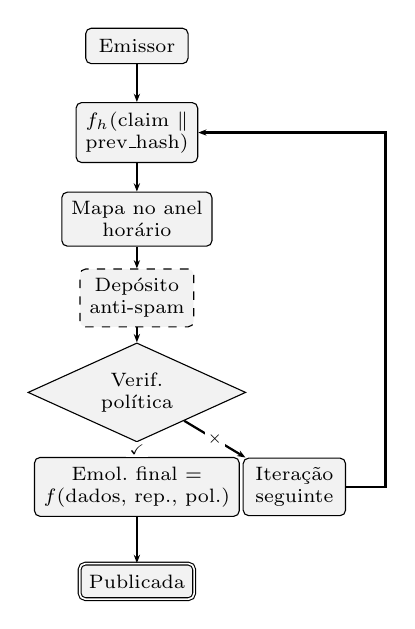
\begin{tikzpicture}[
    box/.style={draw, rounded corners=2pt, minimum width=1.3cm, minimum height=0.45cm, align=center, font=\scriptsize, fill=black!5},
    dec/.style={draw, diamond, aspect=2.2, minimum width=0.9cm, align=center, font=\scriptsize, fill=black!5},
    arr/.style={-{Stealth[length=3pt]}, thick},
    lbl/.style={font=\tiny, fill=white, inner sep=1pt}
]
\node[box] (iss) at (0,0) {Emissor};
\node[box] (hash) at (0,-1.1) {$f_h$(claim $\|$\\prev\_hash)};
\node[box] (ring) at (0,-2.2) {Mapa no anel\\horário};
\node[box, dashed] (spam) at (0,-3.2) {Depósito\\anti-spam};
\node[dec] (check) at (0,-4.4) {Verif.\\política};
\node[box] (rej) at (2,-5.6) {Iteração\\seguinte};
\node[box] (fee) at (0,-5.6) {Emol.\ final =\\$f$(dados, rep., pol.)};
\node[box, double] (pub) at (0,-6.8) {Publicada};

\draw[arr] (iss) -- (hash);
\draw[arr] (hash) -- (ring);
\draw[arr] (ring) -- (spam);
\draw[arr] (spam) -- (check);
\draw[arr] (check) -- node[lbl] {$\times$} (rej);
\draw[arr] (check) -- node[lbl] {\checkmark} (fee);
\draw[arr] (fee) -- (pub);
\draw[arr] (rej.east) -- ++(0.5,0) |- (hash.east);
\end{tikzpicture}
\caption{Protocolo de seleção de verificadores. O depósito anti-spam é opcional e pode ser reembolsável. Os emolumentos finais só são pagos em caso de aceitação.}
\label{fig:verifier}
\end{figure}

Cada rejeição acrescenta a resposta completa do verificador (incluindo motivos e condições) ao documento da alegação, ampliando o seu conteúdo. A partir do documento ampliado, é calculado de forma não determinística um novo hash, que mapeia numa posição diferente do anel e seleciona um verificador diferente. A documentação do caminho completo é obrigatória---o emissor não pode prever nem influenciar o verificador seguinte. Se um verificador ignorar um pedido apesar de uma política declarada compatível, as testemunhas (se presentes) registam-no, e o emissor pode anexar a prova testemunhal aquando da publicação final.

\begin{figure}[ht]
\centering
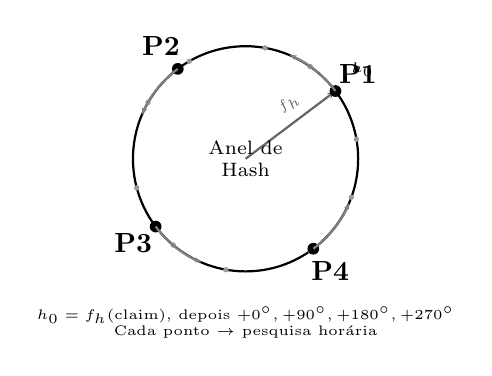
\begin{tikzpicture}[scale=0.65]
% Ring
\draw[thick] (0,0) circle (2.2cm);
% DID nodes on ring
\foreach \a in {10,55,80,120,150,195,230,260,305,340} {
  \fill[black!40] (\a:2.2) circle (1.5pt);
}
% Hash offset arrow pointing to initial position
\draw[-{Stealth[length=3pt]}, thick, black!60] (0,0) -- node[font=\tiny,above,sloped,pos=0.6] {$f_h$} (37:2.2);
\fill[black] (37:2.2) circle (2pt);
\node[font=\tiny,anchor=south west] at (37:2.35) {$h_0$};
% N=4 points offset from h0 by +0, +90, +180, +270
\foreach \offset/\l in {0/P1,90/P2,180/P3,270/P4} {
  \pgfmathsetmacro{\ang}{37+\offset}
  \node[fill=black, circle, inner sep=1.5pt] (p\offset) at (\ang:2.2) {};
  \node[font=\tiny,font=\bfseries] at (\ang:2.75) {\l};
  % clockwise search arc
  \draw[-{Stealth[length=2.5pt]}, thick, gray] (\ang:2.2) arc (\ang:\ang+30:2.2);
}
\node[font=\scriptsize, align=center] at (0,0) {Anel de\\Hash};
\node[font=\tiny, align=center] at (0,-3.2) {$h_0 = f_h(\text{claim})$, depois $+0^{\circ},+90^{\circ},+180^{\circ},+270^{\circ}$\\Cada ponto $\rightarrow$ pesquisa horária};
\end{tikzpicture}
\caption{Seleção multiponto ($N{=}4$). O hash $h_0$ define o desvio; 4 pontos distribuídos uniformemente a partir de $h_0$.}
\label{fig:multipoint}
\end{figure}

\subsection{Protocolo de Testemunho}

O papel de \textbf{Testemunha} confere responsabilização incógnita para a honestidade do verificador através de um protocolo criptográfico de códigos de desafio:

\textbf{Etapa W1.} O requerente assina o pedido de verificação e envia-o a $N_w$ testemunhas---contactos da rede social do requerente ou prestadores especializados de serviços de testemunho que atuam mediante emolumentos.

\textbf{Etapa W2.} Cada testemunha $w_i$ assina todo o pedido assinado, guarda a assinatura original $\sigma_i$ e calcula um código de desafio $c_i = h(\sigma_i)$. O código de desafio é acrescentado ao pedido.

\textbf{Etapa W3.} O pedido, agora transportando $N_w$ códigos de desafio, é enviado ao verificador. O verificador observa os códigos mas \emph{não consegue determinar} quem são as testemunhas nem se os códigos correspondem a assinaturas reais.

\textbf{Etapa W4 (verificador honesto).} Se o verificador responder de acordo com a sua política declarada, os códigos de desafio permanecem opacos. As testemunhas nunca são reveladas. Não é publicado qualquer dado adicional.

\textbf{Etapa W5 (violação de política).} Se o verificador violar a sua política (ignorar o pedido, responder de forma inconsistente), o requerente detém as assinaturas originais $\sigma_i$ das testemunhas. Estas podem ser publicadas como dados complementares: qualquer pessoa pode verificar $c_i = h(\sigma_i)$, provando que a testemunha estava presente. O requerente pode publicar de forma independente---o verificador já assinou os códigos de desafio na sua resposta.

\textbf{A propriedade do bluff.} O requerente pode substituir alguns ou todos os códigos de desafio por valores aleatórios. O verificador não consegue distinguir os códigos genuínos (respaldados por autoridades de elevada reputação) do ruído. Esta \emph{incerteza} é o mecanismo de execução: cada pedido comporta o risco de que uma autoridade respeitada esteja a observar de forma incógnita. O custo de manter esta pressão é praticamente nulo (gerar números aleatórios), ao passo que o custo potencial da desonestidade para o verificador é catastrófico. O comportamento honesto é incentivado mesmo na ausência de testemunhas reais.

\textbf{Autoridade como testemunha.} Uma Autoridade que endossa uma alegação pode combinar serviços de testemunho: ``Endosso a sua alegação e sirvo de testemunha incógnita durante a verificação.'' Trata-se de um modelo de negócio natural---a Autoridade já dispõe do contexto. Contudo, os dois papéis são logicamente independentes.

\subsection{Princípio do Radicalismo Dispendioso}

Três canais de custo somam-se em simultâneo (Fig.~\ref{fig:radicalism}):

\textbf{Canal 1: Custo de Iteração.} Cada rejeição obriga a uma nova iteração que consome tempo e recursos. Crescimento linear.

\textbf{Canal 2: Inchaço do Documento.} Cada iteração acrescenta a resposta completa do verificador ao documento da alegação. O crescimento é linear, mas com um valor de base: a carga inicial (conteúdo da alegação, endosso da autoridade, assinaturas criptográficas) já tem uma dimensão não trivial $B_0$. Dimensão total após $k$ iterações: $S(k) = B_0 + k \cdot \Delta$, onde $\Delta$ é a dimensão média da resposta.

\textbf{Canal 3: Prémio de Risco do Verificador.} O risco é subjetivo. O verificador avalia se as políticas declaradas do DID requerente entram em conflito com os seus próprios interesses comerciais, sociais ou políticos. O prémio pode escalar exponencialmente com a distância percecionada face ao ``ideal'' do verificador: $P(d) = \alpha \cdot e^{\beta d}$, onde $d$ é a métrica de distância subjetiva do verificador. Além de uma fronteira pessoal intransponível, o verificador pode recusar por completo.

\begin{figure}[ht]
\centering
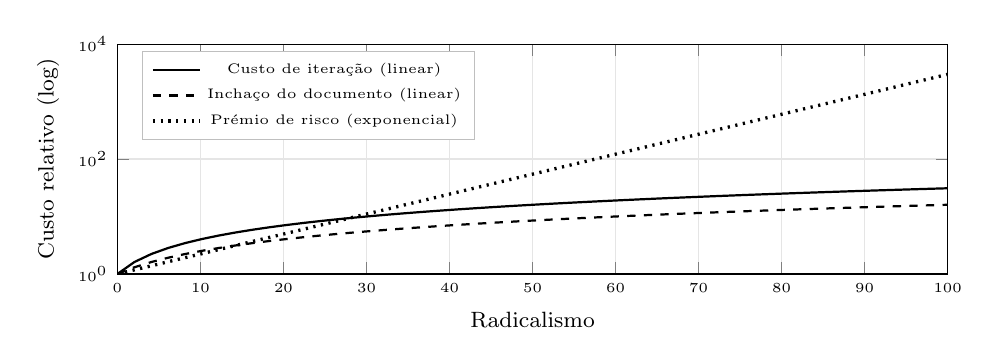
\begin{tikzpicture}
\begin{axis}[
    width=\columnwidth,
    height=4.5cm,
    xlabel={\footnotesize Radicalismo},
    ylabel={\footnotesize Custo relativo (log)},
    ymode=log,
    xmin=0, xmax=100,
    ymin=1, ymax=10000,
    grid=major,
    grid style={gray!20},
    legend style={at={(0.03,0.97)},anchor=north west,font=\tiny,draw=gray!50},
    tick label style={font=\tiny},
    label style={font=\footnotesize},
]
\addplot[black, thick, domain=0:100, samples=50] {1 + 0.3*x};
\addlegendentry{Custo de iteração (linear)}
\addplot[black, thick, dashed, domain=0:100, samples=50] {1 + 0.15*x};
\addlegendentry{Inchaço do documento (linear)}
\addplot[black, thick, dotted, line width=1.2pt, domain=0:100, samples=100] {exp(0.08*x)};
\addlegendentry{Prémio de risco (exponencial)}
\end{axis}
\end{tikzpicture}
\caption{Escalada de custos ao longo de três canais. O prémio de risco domina em níveis elevados de radicalismo.}
\label{fig:radicalism}
\end{figure}

Fundamentalmente, isto não é censura. Nenhuma alegação é proibida. O sistema fixa o preço do risco (Tabela~\ref{tab:costs}).

\begin{table}[ht]
\centering
\caption{Comparação de custos por tipo de alegação.}
\label{tab:costs}
\footnotesize
\begin{tabular}{@{}lcccc@{}}
\toprule
\textbf{Tipo} & \textbf{Iter.} & \textbf{Doc} & \textbf{Emol.} & \textbf{Total} \\
\midrule
Credível & $k_{\min}$ & $B_0$ & $P_{\min}$ & Baixo \\
Controversa & $k_{\text{med}}$ & $B_0{+}k\Delta$ & $\alpha e^{\beta d}$ & Moderado \\
Radical & $k_{\max}$ & $\gg B_0$ & $\gg P_{\min}$ & Muito alto \\
Fraudulenta & $\to\infty$ & --- & --- & Impublicável \\
\bottomrule
\end{tabular}
\end{table}

% ============================================================
% 6. REPUTATION AND RISK
% ============================================================
\section{Avaliação de Reputação e de Risco}

\subsection{Modelo de Acumulação de Reputação}

A reputação exibe três propriedades: \textbf{acumulação lenta} (crescimento incremental através de comportamento consistente), \textbf{destruição rápida} (uma única fraude pode reduzir a pontuação de forma catastrófica) e \textbf{avaliação individual} (cada parte consumidora pode aplicar a sua própria função de agregação).

\subsection{Autoridades Reputáveis}

Uma Autoridade Reputável analisa alegações e, se satisfeita, coassina-as---apostando a sua própria reputação (Fig.~\ref{fig:authority}). A assimetria é intencional: ganhar reputação é lento (incremento de $+\delta$ por cada endosso honesto), ao passo que perdê-la é catastrófico ($-\Delta \gg \delta$ por cada endosso falso; a título ilustrativo, p.\,ex., $+2\%$ contra $-70\%$). A estratégia ótima é sempre rejeitar alegações suspeitas. Os valores concretos de $\delta$ e $\Delta$ são parâmetros do sistema.

\begin{figure}[ht]
\centering
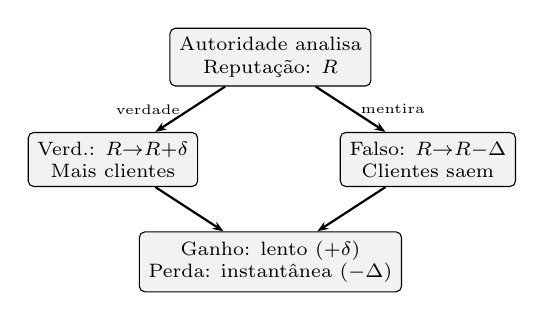
\begin{tikzpicture}[
    box/.style={draw, rounded corners=2pt, minimum width=2cm, minimum height=0.6cm, align=center, font=\scriptsize, fill=black!5},
    arr/.style={-{Stealth[length=4pt]}, thick}
]
\node[box] (exam) at (0,0) {Autoridade analisa\\Reputação: $R$};
\node[box] (true) at (-2,-1.3) {Verd.: $R{\to}R{+}\delta$\\Mais clientes};
\node[box] (false) at (2,-1.3) {Falso: $R{\to}R{-}\Delta$\\Clientes saem};
\node[box] (insight) at (0,-2.6) {Ganho: lento ($+\delta$)\\Perda: instantânea ($-\Delta$)};

\draw[arr] (exam) -- node[left,font=\tiny] {verdade} (true);
\draw[arr] (exam) -- node[right,font=\tiny] {mentira} (false);
\draw[arr] (true) -- (insight);
\draw[arr] (false) -- (insight);
\end{tikzpicture}
\caption{Autoridade Reputável---incentivos assimétricos.}
\label{fig:authority}
\end{figure}

\subsection{Reputação Multidimensional}

A reputação não é um escalar, mas um vetor ao longo de múltiplas dimensões: fiabilidade financeira, integridade pessoal, competência profissional, envolvimento cívico e outras (Fig.~\ref{fig:reputation-radar}). Diferentes prestadores de avaliação projetam este vetor de forma distinta consoante o contexto---um credor prioriza a fiabilidade financeira, um empregador a competência profissional, um vizinho o comportamento cívico. Não existe uma única pontuação de reputação ``correta''; apenas perspetivas.

\begin{figure}[ht]
\centering
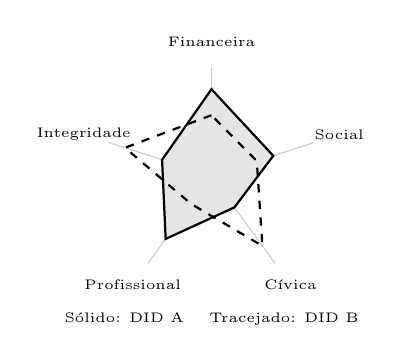
\begin{tikzpicture}[scale=0.55]
\foreach \a/\l in {90/Financeira,162/Integridade,234/Profissional,306/Cívica,18/Social} {
  \draw[gray!40] (0,0) -- (\a:2.5);
  \node[font=\tiny, align=center] at (\a:3.1) {\l};
  \foreach \r in {0.8,1.6,2.4} {
    \fill[black!15] (\a:\r) circle (0.5pt);
  }
}
\draw[thick, fill=black!10] (90:2.0) -- (162:1.2) -- (234:1.8) -- (306:0.9) -- (18:1.5) -- cycle;
\draw[thick, dashed] (90:1.4) -- (162:2.1) -- (234:0.8) -- (306:2.0) -- (18:1.1) -- cycle;
\node[font=\tiny] at (0,-3.3) {Sólido: DID A \quad Tracejado: DID B};
\end{tikzpicture}
\caption{Vetores de reputação multidimensionais. Diferentes DIDs exibem perfis distintos ao longo das dimensões.}
\label{fig:reputation-radar}
\end{figure}

\subsection{Avaliação de Risco Democratizada}

A RSN democratiza a avaliação sistemática de risco---uma capacidade atualmente concentrada nas instituições financeiras mas aplicável muito para além da banca. Conglomerados industriais que avaliam a fiabilidade de fornecedores, seguradoras que fixam o preço do risco comportamental, diligências prévias para fusões e aquisições, estimativa do tempo de vida útil de equipamentos na indústria transformadora---onde quer que o risco de contraparte exija avaliação, a RSN oferece uma alternativa descentralizada e orientada pelo mercado. Um mercado de serviços de interpretação traduz os dados brutos de reputação multidimensional em resumos acionáveis, tornando a avaliação de contrapartes acessível a qualquer participante a custo marginal.

% ============================================================
% 7. CONSENSUS AND DISPUTE RESOLUTION
% ============================================================
\section{Consenso e Resolução de Litígios}

\subsection{Modelo de Justiça Descentralizada}

A RSN reformula a justiça como um problema de negociação bilateral. A ameaça de dano reputacional permanente e verificável é um dissuasor mais eficaz do que um processo judicial que a parte lesada não pode custear.

\subsection{Consenso Emergente}

Cada participante mantém um limiar pessoal de satisfação. O consenso agregado da rede emerge como a média estatística de milhares de negociações bilaterais (Fig.~\ref{fig:consensus}). Uma resposta muito acima do consenso (bárbara) é dispendiosa de publicar. Uma resposta próxima do consenso (proporcional) é barata. O consenso não é uma regra---é um sinal de preço.

\begin{figure}[ht]
\centering
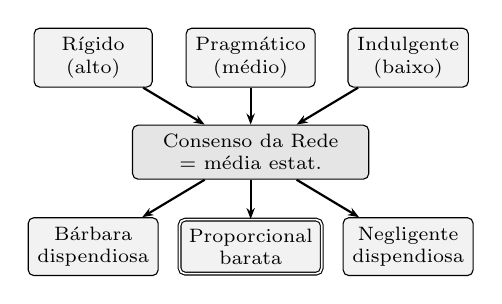
\begin{tikzpicture}[
    person/.style={draw, rounded corners=2pt, minimum width=1.5cm, minimum height=0.5cm, align=center, font=\scriptsize, fill=black!5},
    arr/.style={-{Stealth[length=4pt]}, thick}
]
\node[person] (a) at (-2,0) {Rígido\\(alto)};
\node[person] (b) at (0,0) {Pragmático\\(médio)};
\node[person] (c) at (2,0) {Indulgente\\(baixo)};
\node[person, fill=black!10, minimum width=3cm] (cons) at (0,-1.2) {Consenso da Rede\\= média estat.};
\node[person] (exp) at (-2,-2.4) {Bárbara\\dispendiosa};
\node[person, double] (prop) at (0,-2.4) {Proporcional\\barata};
\node[person] (neg) at (2,-2.4) {Negligente\\dispendiosa};

\draw[arr] (a) -- (cons);
\draw[arr] (b) -- (cons);
\draw[arr] (c) -- (cons);
\draw[arr] (cons) -- (exp);
\draw[arr] (cons) -- (prop);
\draw[arr] (cons) -- (neg);
\end{tikzpicture}
\caption{Consenso emergente a partir de limiares individuais de satisfação.}
\label{fig:consensus}
\end{figure}

\subsection{Calibração da Punição}

Cada Titular de DID declara publicamente as respostas a categorias específicas de má conduta. Declarações desproporcionadamente severas ou brandas atraem sinais reputacionais negativos. Declarações proporcionais são aceites sem fricção---um sistema de punição autocalibrado.

As próprias declarações de consenso estão sujeitas à deteção de hipocrisia: comprometer-se declarativamente com uma posição de consenso mas comportar-se de forma inconsistente constitui uma infração reputacional mais grave do que o desvio subjacente, pois demonstra um engano intencional.

\subsection{Delegação}

Todas as atividades no âmbito de um DID---com uma exceção---podem ser delegadas noutro DID. \textbf{O papel de Sujeito---o DID cujo comportamento a alegação descreve---não pode ser delegado; está intransferivelmente vinculado ao titular de identidade a que a alegação se refere.} Os restantes papéis ativos---Emissor, Autoridade, Testemunha, Verificador---podem ser transferidos para um DID delegado designado, seja para verificação, submissão de alegações, participação no consenso ou resolução de litígios. A delegação é revogável a qualquer momento. Isto permite a especialização (p.\,ex., serviços profissionais de verificação) enquanto o Titular retém o controlo e a responsabilidade últimos. A delegação aplica-se a todo o sistema e é essencial para a escalabilidade.

\subsection{Da Moralidade Individual ao Contrato Social Emergente}

A política declarada de cada DID representa uma formalização da moralidade individual: o que o Titular considera aceitável, como responde a comportamentos específicos, o que exige das contrapartes. Estas políticas não são impostas por um conceptor do sistema---são escolhidas por cada participante e expressas em formato legível por máquina.

Esta formalização possibilita uma emergência em três fases. Primeiro, a moralidade individual é codificada como \textbf{política}---um conjunto de regras declaradas, limiares e funções de resposta que o DID se compromete a cumprir. Segundo, o agregado de todas as políticas da rede produz uma \textbf{ética emergente}---normas estatisticamente observáveis que nenhum participante isolado concebeu, mas que resultam da interação de milhares de posições morais individuais~\cite{durkheim1893}. Terceiro, esta ética emergente, expressa como normas comportamentais partilhadas e reforçada por sinais de preço bilaterais, constitui um \textbf{contrato social mensurável}---não uma construção teórica que ninguém assinou~\cite{rawls1971}, mas um conjunto de regras empiricamente observável e respaldado por comportamento efetivo.

Este processo espelha as conclusões da teoria dos fundamentos morais~\cite{haidt2012}: a moralidade humana é intuitiva, pluralista e culturalmente variável. A RSN não exige consenso moral como entrada; produz consenso comportamental como saída. O contrato social resultante não é estático---evolui à medida que os participantes entram, saem e ajustam as suas políticas em resposta à retroação da rede. Ao contrário da teoria clássica do contrato social, este contrato é revogável, observável e executável sem um soberano.

% ============================================================
% 8. ECONOMIC MODEL
% ============================================================
\section{Modelo Económico}

As secções anteriores descreveram uma ferramenta---os mecanismos de verificação da RSN, a estrutura de custos e o consenso emergente. Esta secção descreve uma metodologia para aplicar essa ferramenta à transição fiscal e de governação. A ferramenta é de uso geral; a metodologia que se segue é uma das aplicações possíveis.

\subsection{Estrutura de Incentivos}

A reputação como capital cria incentivos diretos ao comportamento honesto. Em funcionamento normal, os participantes constroem reputação naturalmente através de transações quotidianas e compromissos cumpridos. A despesa principal recai sobre as alegações \emph{negativas}---o registo de danos causados por outros. Esta assimetria incentiva um comportamento útil e fiável: ser honesto não acarreta custo adicional, ao passo que ser prejudicial cria um rasto documentado que outros pagarão para preservar. A hipocrisia---declarar regras sem as cumprir---é o modo de falha mais dispendioso, pois demonstra um engano intencional.

\subsection{Sistema Fiscal Paralelo}

Três componentes possibilitam a pressão concorrencial: (1)~\textbf{Imposto Simples}---uma única taxa proporcional sem exceções, inicialmente ligeiramente abaixo da taxa efetiva existente; (2)~\textbf{Registo Eletrónico de Despesa (RED)}---invertendo o modelo checo EET para que os cidadãos fiscalizem a despesa do Estado; (3)~\textbf{Afetação de Impostos Dirigida pelo Cidadão}---começando em alguns pontos percentuais no primeiro ano e alcançando, ao fim de uma década, algo entre as dezenas baixas de por cento e uma migração completa para um sistema dirigido pelo cidadão, consoante o ritmo de adoção. O tempo efetivo depende da rapidez com que surgem alternativas de mercado livre aos serviços do Estado e da disposição do Estado para cooperar com a transição; a função do tempo não tem de ser linear, e não há razão para fixar um limite superior ao ponto onde a adoção pode acabar por chegar.

% ============================================================
% 9. MIGRATION PATH
% ============================================================
\section{Caminho de Migração}

A migração processa-se em três fases (Fig.~\ref{fig:migration}): \textbf{Fase~1: Sobreposição} (a RSN como camada informacional, o Estado é o único prestador), \textbf{Fase~2: Concorrência} (a RSN oferece alternativas funcionais, uso de duplo sistema) e \textbf{Fase~3: Transição} (a RSN supera os equivalentes estatais, migração voluntária). A transição é reversível em todas as fases.

\begin{figure}[ht]
\centering
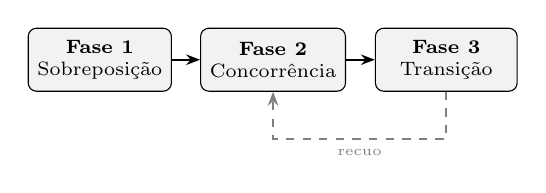
\begin{tikzpicture}[
    phase/.style={draw, rounded corners=3pt, minimum width=1.8cm, minimum height=0.8cm, align=center, font=\scriptsize, fill=black!5},
    arr/.style={-{Stealth[length=5pt]}, thick}
]
\node[phase] (p1) at (0,0) {\textbf{Fase 1}\\Sobreposição};
\node[phase] (p2) at (2.2,0) {\textbf{Fase 2}\\Concorrência};
\node[phase] (p3) at (4.4,0) {\textbf{Fase 3}\\Transição};

\draw[arr] (p1) -- (p2);
\draw[arr] (p2) -- (p3);
\draw[arr, dashed, gray] (p3.south) -- ++(0,-0.6) -| node[below,font=\tiny,pos=0.25] {recuo} (p2.south);
\end{tikzpicture}
\caption{Migração em três fases---reversível em todas as fases.}
\label{fig:migration}
\end{figure}

O principal mecanismo de pressão é fiscal: quando os contribuintes condicionais atingem uma ``minoria economicamente significativa $X$''---um grupo suficientemente grande para que a repressão contra ele cause danos económicos não triviais e a desobediência civil se torne uma ameaça credível---o Estado entra em negociação. A título ilustrativo, usamos $X \approx 15\%$ do PIB, mas o limiar efetivo depende da economia específica.

% ============================================================
% 10. SECURITY ANALYSIS
% ============================================================
\section{Análise de Segurança}

Consideramos cinco categorias de adversários: maus atores individuais, grupos organizados, adversários empresariais, adversários ao nível do Estado e adversários ao nível do protocolo.

\textbf{Resistência a Sybil}~\cite{douceur2002}. Construir reputação exige uma interação sustentada e verificável. O custo de um ataque Sybil bem-sucedido cresce linearmente com o número de identidades falsas e quadraticamente com o nível de reputação-alvo. Operar múltiplos DIDs em paralelo é possível mas dispendioso por conceção---cada identidade tem de acumular reputação de forma independente através de atividade genuína. Nas sociedades livres, este custo dissuade o abuso ocasional; nas ditaduras, os DIDs paralelos tornam-se uma ferramenta de sobrevivência que possibilita uma resistência compartimentada, a coordenação clandestina e uma navegação mais segura no mercado negro.

\textbf{Defesa contra conluio.} Os padrões de endosso mútuo entre grupos fechados são detetáveis através da análise do grafo social. As funções de agregação de reputação descontam as alegações provenientes de fontes densamente agrupadas.

\textbf{Adversário ao nível do Estado.} O encaminhamento onion, a ausência de infraestrutura centralizada e a distribuição do papel de Verificador por toda a base de participantes garantem que a supressão exige medidas desproporcionadas face a qualquer benefício.

\textbf{Privacidade vs.\ responsabilização.} A pseudonímia---um meio-termo entre o anonimato e a divulgação de identidade---permite que os DIDs acumulem reputação significativa sem revelar a identidade real do Titular.

% ============================================================
% 11. PRIVACY
% ============================================================
\section{Considerações de Privacidade}

O modelo de privacidade da RSN assenta na pseudonímia. O Titular controla a divulgação de identidade: mínima (pseudónimo puro), seletiva (credenciais específicas associadas) ou total (identidade legal associada). As alegações publicadas são permanentes---o sistema suporta a correção contextual mas não o apagamento. Um Titular pode abandonar um DID comprometido e recomeçar, abdicando da reputação acumulada.

% ============================================================
% 12. RELATED WORK
% ============================================================
\section{Trabalho Relacionado}

A especificação W3C DID Core~\cite{did2022} e a Ceramic Network~\cite{ceramic2023} fornecem a base de identidade. O EigenTrust~\cite{kamvar2003} demonstrou a agregação distribuída de reputação sem autoridade central. Os SBTs~\cite{weyl2022} introduziram tokens sociais intransferíveis. A RSN distingue-se pela ênfase no custo económico como filtro de qualidade e pelo seu mecanismo de fixação do preço do radicalismo.

As DAOs~\cite{buterin2014} e o voto quadrático~\cite{buterin2019} demonstraram a viabilidade da governação descentralizada. A RSN deriva o consenso de negociações bilaterais de preço, em vez do voto.

A proposta apoia-se na teoria anarcocapitalista~\cite{rothbard1973,hoppe2001} para a prestação privada de serviços, mas afasta-se dela em dois aspetos críticos: é concebida para o rancor e os impulsos retributivos em vez de pressupor racionalidade, e propõe uma transição gradual em vez de uma revolução. O conceito de contratos sociais emergentes tem antecedentes na teoria da ordem espontânea de Hayek~\cite{hayek1973}.

\textbf{Anarco-agorismo.} A RSN partilha um terreno comum significativo com a contraeconomia agorista~\cite{konkin2006}---em particular a ênfase na construção de instituições paralelas e na troca voluntária. Contudo, o agorismo tende a pressupor o autointeresse racional como mecanismo de coordenação suficiente e carece frequentemente de um caminho de migração concreto a partir das estruturas estatais existentes. A RSN incorpora explicitamente tendências comportamentais não racionais e fornece um mecanismo de pressão fiscal para uma transição gradual.

\textbf{Meritocracia.} A RSN pode representar uma primeira descrição funcional de como a meritocracia~\cite{young1958} pode emergir como propriedade sistémica, e não como um slogan. Os sistemas meritocráticos tradicionais falham porque exigem uma autoridade central para definir e fazer valer o ``mérito''. Na RSN, o mérito emerge de avaliações bilaterais: quem entrega valor acumula reputação; nenhum comité decide quem tem mérito.

\textbf{Propriedade como privilégio.} A RSN afasta-se fundamentalmente do tratamento anarcocapitalista e da escola austríaca dos direitos de propriedade como naturais e absolutos. No quadro da RSN, a propriedade é um \emph{privilégio}---um reconhecimento social que pode, em casos extremos, ser retirado pela comunidade quando um participante viola fundamentalmente as normas partilhadas (traição, recusa de defender a comunidade numa crise existencial, exploração sistemática). Não se trata de expropriação estatal, mas da retirada do reconhecimento social pela rede de relações bilaterais.

% ============================================================
% 13. LIMITATIONS
% ============================================================
\section{Discussão e Limitações}

\textbf{Arranque a frio.} O valor da RSN depende de efeitos de rede; os primeiros aderentes deparam-se com um valor limitado até que a participação atinja um limiar. Contudo, mesmo em fases iniciais, a rede DID serve de fonte de informação complementar útil. Espera-se que a avaliação inicial de reputação e a avaliação de autoridades se desenvolvam gradualmente, com sofisticação crescente.

\textbf{Anti-parasitagem e controlo de acesso.} Os DIDs-alvo podem impor emolumentos graduais e restrições de acesso às consultas de DIDs de baixa reputação. Não se trata de uma escala binária, mas contínua: quanto menos reputação um DID consulente tiver, menos informação recebe, mais tempo espera e mais paga. Este mecanismo incentiva a participação genuína em detrimento do consumo passivo.

\textbf{Desigualdade no acesso.} O custo de publicar alegações pode filtrar queixas legítimas de participantes economicamente desfavorecidos. Mitigação: cada participante serve simultaneamente de potencial verificador (ou delega esse papel) e aufere emolumentos de verificação. Ao longo de um horizonte temporal suficiente, um participante não radical deverá aproximar-se da neutralidade financeira---o rendimento de verificação a compensar aproximadamente os custos de publicação. Trata-se de uma expectativa estatística, não de uma garantia.

\textbf{Desigualdade de reputação.} Os primeiros aderentes acumulam vantagens que podem criar barreiras para os que chegam mais tarde. Contudo, a avaliação de reputação é realizada por prestadores terceiros que podem optar por atenuar a vantagem do primeiro entrante através dos seus algoritmos de agregação. Ser o primeiro com boa reputação é uma vantagem económica comparativa legítima---e isso é intencional.

\textbf{Questões em aberto.} As funções de custo ótimas, as normas de agregação, a governação do protocolo e a interação com dados de reputação sintética gerados por IA continuam a ser áreas para trabalho futuro.

Este artigo não afirma que a RSN produzirá resultados ótimos em todas as circunstâncias. Afirma que a RSN representa uma alternativa \emph{viável}---tecnicamente implementável, economicamente autossustentável e socialmente compatível com as tendências comportamentais humanas tal como elas realmente são.

% ============================================================
% 14. CONCLUSION
% ============================================================
\section{Conclusão}

Este artigo apresentou a Rede Social de Reputação, um protocolo descentralizado que possibilita a troca de reputação pseudónima e verificável. O Princípio do Radicalismo Dispendioso garante que as alegações fraudulentas ficam com um preço proibitivo sem censura. O caminho de migração proposto possibilita uma transição gradual e reversível a partir das instituições existentes. A conceção incorpora a natureza humana tal como ela é---incluindo a mesquinhez, o rancor e o desejo de satisfação retributiva---em vez de exigir uma transformação ideológica. O resultado não é uma utopia, mas um sistema em que a justiça é acessível, a reputação é conquistada e o custo da má conduta é suportado pela parte que a causou.

% ============================================================
% REFERENCES
% ============================================================
\bibliography{references}

\end{document}
